%% Copyright Roberto Di Cosmo, Jun Furuse, Didier Remy, and Pierre Weis
%% All rights reserved.

%% $Id$

\documentclass[12pt]{article}

% You need graphics package
\usepackage{../doc/manual}
\usepackage{color}
\usepackage{xwindows-colors}
\usepackage{graphicx}
\usepackage{advi-graphicx}
\usepackage{alltt}

\usepackage{pst-all}

%% advi must occur after packages using PStricks macros 
%% (it redefines some of them) 
\usepackage{advi}
\usepackage{advi-annot}

\usepackage{hyperref}

\def\mathsym#1{\ifmmode{#1}\else$#1$\fi}

\pagestyle{empty}

\definecolor{red}{rgb}{1.0,0.0,0.0}
\definecolor{green}{rgb}{0.0,1.0,0.0}
\definecolor{blue}{rgb}{0.0,0.0,1.0}
\definecolor{lightblue}{rgb}{0.6784,0.8471,0.9020}
\definecolor{c1}{rgb}{1.0,0.0,0.0}
\definecolor{c2}{rgb}{0.5,0.4,0.0}
\definecolor{c3}{rgb}{0.0,0.8,0.0}
\definecolor{c4}{rgb}{0.0,0.4,0.5}
\definecolor{c5}{rgb}{0.0,0.0,1.0}
\definecolor{c6}{rgb}{0.5,0.0,0.5}

\def\smallpause{0.3}

\def\keymenu#1{\textcolor{red}{\underline{#1}}}

\def\advifooter{\vbox to 0em{\vbox to \vsize {\vfill
Press: \keymenu{n}ext page \keymenu{p}revious page
\keymenu{\textvisiblespace} next pause%
\hfill{\adviembed[sticky = advianim, width = 1.56cm, height = 1.824cm]{animate -geometry @g! -window @p advilogo.anim.gif}}
} \vss}}

\def\adviheader{\noindent
{\bf\Large \ActiveDVI}\\

\includegraphics[width = \textwidth]{bar.eps}}

\let \Newpage \newpage
\def \newpage {\Newpage \advifooter\adviheader}

\def\adviemptyfooter{\vbox to 0em{\vbox to \vsize {\vfill
~~\vss\advikillembed{advianim}}}}

\def\lastpage{\Newpage\adviemptyfooter\adviheader}

%  \setlength\textwidth{660\p@}
%  \setlength\textheight{460\p@}

\begin{document}

% We use the default mode of advi that considers white as transparent
% as if \epstransparent has been evaluated.

\newpage

\subsection* {Modifying the page backround}

You can modify the background of your presentations:
  \begin{itemize}
    \item define the background color
    \item define a function to be run on the background (this is
    limited to a few color gradients, but it can be expanded to more
    sophisticated effects) 
    \item add a background image (which can be alpha-blended on top of
    the background color).
  \end{itemize}

If these options are used \emph{together}, they are applied in this
order: first solid background color, then gradient function, then
image drawing.\\

This file is a simple showcase for the current background effects.

\newpage

\tableofcontents

\newpage

\section{Setting the background color}

This page has a yellow background because we included
in the {\LaTeX} source of the page the following command:

\begin{quote}
  \begin{verbatim}
  \advibg{color = yellow} 
  \end{verbatim}
\end{quote}
\advibg{color = yellow} 

\newpage

{\color[named]{Goldenrod}{
\section{Setting the background color: gradients}

By choosing one of the \verb|hgradient|, \verb|vgradient|,
\verb|d1gradient|, \verb|d2gradient|, \verb|cgradient|, or
\verb|circgradient| predefined functions, we convert the plain
background color into a color gradient from the chosen color to white
(by default).

In fact, the gradient color bounds can be precised with fields:

\begin{itemize}
 \item \verb"colorstart" to specify the starting color of the gradient,
 \item \verb"colorstop" to specify the ending color of the gradient.
\end{itemize}

When left unspecified, those colors respectively default to
\verb"white" and the background color.

You specify the area where the gradient is drawn by giving the
coordinates of the rectangle that defines the area:
\begin{itemize}
\item \verb"xstart" and \verb"ystart" define the lower left point of the area,
\item \verb"width" and \verb"height" specify the width and height of
the area.
\end{itemize}

When left unspecified, the gradient's area defaults to the entire page.

Area dimension specifications are floating point numbers in the range
\verb|[0 .. 1]|. Each number gives the ratio of the specified
dimension with respect to the corresponding page dimension (hence $0$
means a null dimension and $1$ means the entire actual page relevant
dimension).

For centered or circular gradient, the fields \verb"xcenter" and
\verb"ycenter" define the coordinates of the center point of the
gradient into the gradient area (the \verb"xcenter" and \verb"ycenter"
specifications use the same convention as in the preceding paragraph:
a ratio of a given dimension, in this case a ratio of the gradient
area's width and height respectively).

When left unspecified, the gradient's center defaults to the center of
its area.

\vfill

The command to obtain this background is:

\advibg{color = [named]{CadetBlue}}

\begin{quote}
  \begin{verbatim}
  \advibg{color = [named]{CadetBlue}} 
  \end{verbatim}
\end{quote}
\vfill
}}
\newpage

\vfill
\subsection{Horizontal gradient}
\vfill

The command to obtain this background is:

\begin{quote}
  \begin{verbatim}
  \advibg{color = yellow, gradient = "hgradient"} 
  \end{verbatim}
\end{quote}
\advibg{color = yellow, gradient = "hgradient"} 
\vfill

\newpage

\vfill
\subsection{Vertical gradient}
\vfill

The command to obtain this background is:

\advibg{color = blue, gradient = "vgradient"} 

\begin{quote}
  \begin{verbatim}
  \advibg{color = blue, gradient = "vgradient"} 
  \end{verbatim}
\end{quote}
\vfill

\newpage

\vfill
\subsection{First diagonal gradient}
\vfill

The command to obtain this background is:

\advibg{color = green, gradient = "d1gradient"} 

\begin{quote}
  \begin{verbatim}
  \advibg{color = green, gradient = "d1gradient"} 
  \end{verbatim}
\end{quote}
\vfill

\newpage

\vfill
\subsection{Second diagonal gradient}
\vfill

The command to obtain this background is:

\advibg{color = green, gradient = "d2gradient"} 

\begin{quote}
  \begin{verbatim}
  \advibg{color = green, gradient = "d2gradient"} 
  \end{verbatim}
\end{quote}
\vfill

\newpage

\vfill
\subsection{Centered gradient}
\vfill

The command to obtain this background is:

\advibg{color = green, gradient = "cgradient"} 

\begin{quote}
  \begin{verbatim}
  \advibg{color = green, gradient = "cgradient"} 
  \end{verbatim}
\end{quote}
\vfill

\newpage

\vfill
\subsection{Circular gradient}
\vfill

The command to obtain this background is:

\advibg{color = green, gradient = "circgradient"} 

\begin{quote}
  \begin{verbatim}
  \advibg{color = green, gradient = "circgradient"} 
  \end{verbatim}
\end{quote}
\vfill

\newpage

\vfill
\subsection{Circular gradient with starting color}
\vfill

The command to obtain this background is:

\advibg{color = green, gradient = "circgradient",
        colorstart = red}

\begin{quote}
  \begin{verbatim}
  \advibg{color = green, gradient = "circgradient",
          colorstart = "red"} 
  \end{verbatim}
\end{quote}
\vfill

\newpage

\vfill
\subsection{Centered gradient with starting color}
\vfill

The command to obtain this background is:

\advibg{color = green, gradient = "cgradient",
        colorstart = blue}

\begin{quote}
  \begin{verbatim}
  \advibg{color = green, gradient = "cgradient",
          colorstart = "blue"} 
  \end{verbatim}
\end{quote}
\vfill


\newpage

\vfill
\subsection{Small centered gradient with starting color}
\vfill

The command to obtain this background is:

\advibg{color = green, gradient = "cgradient",
        colorstart = blue,
        colorstop = red,
        xcenter = 0.25,
        ycenter = 0.5,
        xstart = 0.5,
        ystart = 0.5,
        width = 0.1,
        height = 0.5}

\begin{quote}
  \begin{verbatim}
    \advibg{color = green, gradient = "cgradient",
            colorstart = blue,
            colorstop = red,
            xcenter = 0.25,
            ycenter = 0.5,
            xstart = 0.5,
            ystart = 0.5,
            width = 0.1,
            height = 0.5}
  \end{verbatim}
\end{quote}
\vfill

\newpage

\vfill
\subsection{Circular gradient with red starting color}
\vfill

The command to obtain this background is:

\advibg{color = [named]{MistyRose},
        gradient = "circgradient",
        colorstart = red,
        colorstop = [named]{MistyRose},
        width = 0.2,
        height = 0.15,
        xstart = 0.75,
        ystart = 0.8,
        xcenter = 0.5,
        ycenter = 0.5}

\begin{quote}
  \begin{verbatim}
\advibg{color = [named]{MistyRose}, gradient = "circgradient",
        colorstart = red,
        colorstop = [named]{MistyRose},
        width = 0.2,
        height = 0.15,
        xstart = 0.75,
        ystart = 0.8,
        xcenter = 0.1,
        ycenter = 0.5}
  \end{verbatim}
\end{quote}
\vfill

\newpage

\section{Setting the background image}

\advibg{image = "world.jpg"} 

We can use an image as background.
This page's background is made of \verb|world.jpg| which
is in the test directory. The source of this page contains

  \begin{quote}
    \begin{verbatim}
    \advibg{image = "world.jpg"} 
    \end{verbatim}
  \end{quote}

\parindent 0pt Note: the image formats supported depend on the variable
  \begin{quote}
CAMLIMAGESLIBS
  \end{quote}
in your Advi's Makefile.config .
\newpage

\section{Positioning the background image}

As documented in the manual, the {\LaTeX} macro for backgrounds has a
wealth of options.\\
For example, there are several different ways to adapt an image to the
size of the background to fill, and they are declared with the
\dockey{fit}{} parameter to \verb|\advibg|:

\dockey[auto]{fit}{fit style}

\begin{quote}

Fit the background image according to \docid{style}, which may only be 
{\tt auto} or one of the following keywords:

\begin{center}
\tt auto \hfill {\rm or} \hfill
\begin{tabular}{l@{\qquad}c@{\qquad}r}
topleft&   top& topright\\
left&  center&  right \\
bottomleft& bottom & bottomright\\
\end{tabular}
\end{center}

The {\tt auto} fit mode means scale the image as desired in both directions
so that it fits the page. The other styles only allows the same scaling
factor in both directions:

\begin {itemize}

\item Corner-styles mean adjust the image in the corner and scale so
that all the page is covered.

\item {\tt center} means scale the image so that all the page is
covered and center it on the page.

\item Segment-styles mean adjust the image and the page on the segment
(in which case, the image may not totally cover the page on the
opposite side).

\end {itemize}

\end{quote}

\framebox{Here come several slides meant to show the effect of these settings.}

\newpage
\vfill
{\Huge Automatic fit (default)}
\vfill
This is obtained by not setting the \dockey{fit}{} parameter:\\
\advibg{image = "world.jpg"}
\begin{center}
  \begin{verbatim}
  \advibg{image = "world.jpg"}
  \end{verbatim}
\end{center}
\vfill
Resize the display window to see how this positioning option works.
\vfill

\newpage

\newcommand{\ttadvibg}{$\backslash$advibg}
\newcommand{\docfit}[1]{\vfill%
The command to obtain this background is:\\%
\begin{center}
{#1}
\end{center}
\vfill%
Resize the display window to see how this positioning option works.%
\vfill%
}

\vfill
{\Huge Top}
\advibg{image = "world.jpg", fit = top}
\docfit{\tt \ttadvibg\{image = "world.jpg", fit = top\}}
\newpage

\vfill
{\Huge Bottom}
\advibg{image = "world.jpg", fit = bottom}
\docfit{\tt \ttadvibg\{image = "world.jpg", fit = bottom\}}

\newpage

\vfill
{\Huge Left}
\advibg{image = "world.jpg", fit = left}
\docfit{\tt \ttadvibg\{image = "world.jpg", fit = left\}}

\newpage

\vfill
{\Huge Right}
\advibg{image = "world.jpg", fit = right}
\docfit{\tt \ttadvibg\{image = "world.jpg", fit = right\}}

\newpage

\vfill
{\Huge Center}
\advibg{image = "world.jpg", fit = center}
\docfit{\tt \ttadvibg\{image = "world.jpg", fit = center\}}

\newpage

\vfill
{\Huge TopLeft}
\advibg{image = "world.jpg", fit = topleft}
\docfit{\tt \ttadvibg\{image = "world.jpg", fit = topleft\}}

\newpage

\vfill
{\Huge TopRight}
\advibg{image = "world.jpg", fit = topright}
\docfit{\tt \ttadvibg\{image = "world.jpg", fit = topright\}}

\newpage

\vfill
{\Huge BottomLeft}
\advibg{image = "world.jpg", fit = bottomleft}
\docfit{\tt \ttadvibg\{image = "world.jpg", fit = bottomleft\}}

\newpage

\vfill
{\Huge BottomRight}
\advibg{image = "world.jpg", fit = bottomright}
\docfit{\tt \ttadvibg\{image = "world.jpg", fit = bottomright\}}

\newpage

\section{Alpha factor and blending}
\dockey[none]{alpha}{float}
\begin{quote}
Set the alpha factor for the background image to \docid{float}
(\doctt{none} means unset).
\end{quote}

\dockey[none]{blend}{blend mode}
\begin{quote}
Set the blend mode to \docid{blend mode}, which should be one of the
following: {\tt normal}, {\tt multiply}, {\tt screen},
{\tt overlay}, {\tt dodge}, {\tt burn}, {\tt darken},
{\tt lighten}, {\tt difference}, {\tt exclusion}, and {\tt none}
(\doctt{none} means unset).
\end{quote}

\framebox{Here are a few example slides}
\newpage

\bigskip

\def\exampleimage{
 {
\includegraphics[width = \textwidth]{bar.eps}}
 {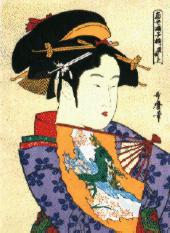
\includegraphics[width = 0.2\textwidth]{dojojismall.jpg}}
}

{\large Normal mode}

{\setblend{normal}{\exampleimage}}

{\large Multiply mode}

{\setblend{multiply}{\exampleimage}}

{\large Screen mode}

{\setblend{screen}{\exampleimage}}

\advibg{color = lightgray} 

\newpage

\bigskip

{\large Overlay mode}

{\setblend{overlay}{\exampleimage}}

{\large Dodge mode}

{\setblend{dodge}{\exampleimage}}

{\large Burn mode}

{\setblend{burn}{\exampleimage}}

\advibg{color = lightgray} 

\newpage

\bigskip

{\large Darken mode}

{\setblend{darken}{\exampleimage}}

{\large Lighten mode}

{\setblend{lighten}{\exampleimage}}

\advibg{color = lightgray} 

\newpage

\bigskip

{\large Difference mode}

{\setblend{difference}{\exampleimage}}

{\large Exclusion mode}

{\setblend{exclusion}{\exampleimage}}

\advibg{color = lightgray} 

\newpage

\vfill
{\Huge Alpha channel}
\vfill
In this page, the background is filled with an image for which we
specify an alpha value of less than 1.\\ 
Notice that this effect is nice, but expensive to realize.

The command to obtain this background is:

\begin{center}
{\tt \char`\\advibg\{alpha = 0.25, image = "dojoji.gif"\}}
\end{center}
\advibg{alpha = 0.25, image = "dojoji.gif"}
\vfill

\newpage

\vfill
{\Huge Blending with a color background}
\vfill
In this page, the background is first set to light blue, then blended
in {\tt difference} mode with the image which is scaled to fit the
available area.\\

The command to obtain this background is:

\advibg{color = lightblue, alpha = 0.1,
        blend = difference,
        image = "dojoji.gif"} 
\begin{center}
{\tt \char`\\advibg\{color = lightblue, alpha = 0.1,
                     blend = difference,
                     image = "dojoji.gif"\}}
\end{center}
\vfill

\Newpage

\advibg{color = black}

{\color{white}
\advifooter\adviheader

\section{Reverse video effect}

If you want a reverse video effect, you just have to set the background
of the page to black and the text color to white, as follows:

\begin{itemize}

\item set the background to black, anywhere in the text of the slide with

\begin{quote}
  \begin{verbatim}
  \advibg{color = black} 
  \end{verbatim}
\end{quote}

\item set the text color of the entire page to white, by putting the
text of the page between in the scope of a \verb"\color" macro call:
\begin{quote}
  \begin{verbatim}
  {\color{white}
   Text of the page
  }
  \end{verbatim}
\end{quote}

\end{itemize}

Write \verb"\advibg{none}" at the beginning of the next slide, if you
want to revert to normal background.

}

\newpage

\advibg{none}

\section{Backgrounds Gallery}

\vfill
{\Huge Solid color background}
\vfill

The command to obtain this background is:

\advibg{color = cyan}

\begin{center}
\begin{verbatim}
  \advibg{color = cyan}
\end{verbatim}
\end{center}
\vfill

\newpage

\vfill
{\Huge Solid color\\ with vertical gradient}
\vfill

The command to obtain this background is:

\advibg{color = cyan, gradient = "vgradient"}

\begin{center}
\begin{verbatim}
  \advibg{color = cyan, gradient = "vgradient"}
\end{verbatim}
\end{center}
\vfill

\newpage

\vfill
{\Huge Vertical gradient\\ with blended image ($\alpha = 0.1$)}
\vfill

The command to obtain this background is:

\advibg{alpha = "0.1", image = "dojoji.gif",
        color = cyan, gradient = "vgradient"}

\begin{center}
\begin{verbatim}
  \advibg{alpha = "0.1", image = "dojoji.gif",
          color = cyan, gradient = "vgradient"}
\end{verbatim}
\end{center}
\vfill

\newpage

\vfill
{\Huge Vertical gradient\\ with blended image ($\alpha = 0.2$)}
\vfill

The command to obtain this background is:

\advibg{alpha = "0.2", image = "dojoji.gif",
        color = cyan, gradient = "vgradient"}

\begin{center}
\begin{verbatim}
  \advibg{alpha = "0.2", image = "dojoji.gif",
          color = cyan, gradient = "vgradient"}
\end{verbatim}
\end{center}
\vfill

\newpage

\vfill
{\Huge Vertical gradient\\ with blended image ($\alpha = 0.4$)}
\vfill

The command to obtain this background is:

\advibg{alpha = "0.4", image = "dojoji.gif",
        color = cyan, gradient = "vgradient"}

\begin{center}
\begin{verbatim}
  \advibg{alpha = "0.4", image = "dojoji.gif",
          color = cyan, gradient = "vgradient"}
\end{verbatim}
\end{center}
\vfill

\newpage

\vfill
{\Huge Vertical gradient\\ with blended image ($\alpha = 0.8$)}
\vfill

The command to obtain this background is:

\advibg{alpha = "0.8", image = "dojoji.gif",
        color = cyan, gradient = "vgradient"}

\begin{center}
\begin{verbatim}
  \advibg{alpha = "0.8", image = "dojoji.gif",
          color = cyan, gradient = "vgradient"}
\end{verbatim}
\end{center}
\vfill

\newpage

\vfill
{\Huge Red circular gradient\\ with blended image ($\alpha = 0.25$)}
\vfill

The command to obtain this background is:

\advibg{color = [named]{LemonChiffon},
        gradient = circgradient,
        colorstart = red,
        image = "dojoji.gif", alpha = 0.25}

\begin{center}
\begin{verbatim}
  \advibg{color = [named]{LemonChiffon},
          gradient = circgradient,
          colorstart = red,
          image = "dojoji.gif", alpha = 0.25}
\end{verbatim}
\end{center}
\vfill

\newpage

\vfill
{\Huge Horizontal red gradient\\ with blended image ($\alpha = 0.25$)}
\vfill

The command to obtain this background is:

\advibg{color = [named]{LemonChiffon},
        gradient = hgradient,
        colorstart = red,
        xstart = 0, ystart = 0,
        width = 0.14, height = 1.,
        image = "dojoji.gif", alpha = 0.25}

\begin{center}
\begin{verbatim}
  \advibg{color = [named]{LemonChiffon},
          gradient = hgradient,
          colorstart = red, xstart = 0, ystart = 0,
          width = 0.14, height = 1.,
          image = "dojoji.gif", alpha = 0.25}
\end{verbatim}
\end{center}
\vfill

\newpage

\vfill
{\Huge Horizontal gradient\\ with solid white}
\vfill

The command to obtain this background is:

\advibg{color = white,
        gradient = hgradient,
        colorstart = blue, colorstop = green,
        xstart = 0, ystart = 0,
        width = 0.14, height = 1.}

\begin{center}
\begin{verbatim}
  \advibg{color = white},
          gradient = hgradient,
          colorstart = blue, colorstop = green,
          xstart = 0, ystart = 0,
          width = 0.14, height = 1.}
\end{verbatim}
\end{center}
\vfill

\newpage

\vfill
{\Huge Horizontal gradient\\ with LemonChiffon}
\vfill

The command to obtain this background is:

\advibg{color = [named]{LemonChiffon},
       gradient = hgradient,
       colorstart = blue, colorstop = green,
       xstart = 0, ystart = 0,
       width = 0.14, height = 1.}

\begin{center}
\begin{verbatim}
  \advibg{color = [named]{LemonChiffon},
          gradient = hgradient,
          colorstart = blue, colorstop = green,
          xstart = 0, ystart = 0,
          width = 0.14, height = 1.}
\end{verbatim}
\end{center}
\vfill

\newpage

\vfill
{\Huge Horizontal gradient\\ with LemonChiffon\\
       and blended image ($\alpha = 0.25$)}
\vfill

The command to obtain this background is:

\advibg{color = [named]{LemonChiffon},
       gradient = hgradient,
       colorstart = blue, colorstop = green,
       xstart = 0, ystart = 0,
       width = 0.14, height = 1.,
      image = "dojoji.gif", alpha = 0.25}

\begin{center}
\begin{verbatim}
  \advibg{color = [named]{LemonChiffon},
          gradient = hgradient,
          colorstart = blue, colorstop = green,
          xstart = 0, ystart = 0,
          width = 0.14, height = 1.,
          image = "dojoji.gif", alpha = 0.25}
\end{verbatim}
\end{center}
\vfill

\newpage

\section{Future work}

  \begin{itemize}
    \item background preferences are ``asynchronous'', in the sense
that they can imply rendering modifications in a part of the page that
has already been displayed; this is why we first scan a page, looking
for background specials (example, a red background), and only after we
render it (setting the background to red before everything else). By
the way, this mechanism was already in place to handle PostScript
headers, that also appear asynchronously.

    \item is it worthwhile to consider the possibility of making a
``synchronous'' variant? This would allow for example to change the
background color after a pause. But at what price ?

    \item anybody willing to add support for color gradients?\\Done.

    \item anybody willing to improve gradients so that we can have
images above a color gradient ?\\Done.

    \item anybody willing to improve gradients so that we can define a
sub window where the color gradient takes place ?\\Done.

    \item anybody willing to improve gradients to a more general
scheme that could be programmable ?

  \end{itemize}
\vfill

The command to obtain this background is:

\advibg{color = cyan, image = "dojoji.gif",
        alpha = 0.25}

\begin{center}
\begin{verbatim}
  \advibg{color = cyan, image = "dojoji.gif",
          alpha = 0.25}
\end{verbatim}
\end{center}
\vfill

\lastpage

~\vfill
\begin{center}

\includegraphics[width=0.5\textwidth]{../tex/advilogo.eps}\\
{\Large \bf That's all, folks!!}
\end{center}
\vfill

\end{document}
